\documentclass[final]{fhnwreport}       %[mode] = draft or final
                                        %{class} = fhnwreport, article, 
                                        %          report, book, beamer, standalone
%%---Main Packages-----------------------------------------------------------------------
\usepackage[english, ngerman]{babel}	%Mul­tilin­gual sup­port for LaTeX
\usepackage[T1]{fontenc}				%Stan­dard pack­age for se­lect­ing font en­cod­ings
\usepackage[utf8]{inputenc}				%Ac­cept dif­fer­ent in­put en­cod­ings
\usepackage{lmodern}                    %The newer Font-Set
\usepackage{textcomp}					%LaTeX sup­port for the Text Com­pan­ion fonts
\usepackage{caption}					%Customising captions in floating environments
\usepackage{graphicx} 					%En­hanced sup­port for graph­ics
\usepackage{float}						%Im­proved in­ter­face for float­ing ob­jects
\usepackage{ifdraft}                    %Let you check if the doc is in draft mode

%%---Useful Packages---------------------------------------------------------------------
\usepackage{color}						%Colour control for LaTeX documents
\usepackage[pdftex,dvipsnames]{xcolor}  %Driver-in­de­pen­dent color ex­ten­sions for LaTeX
\usepackage{csquotes}                   %Simpler quoting with \enquote{}
\usepackage{siunitx} 					%A com­pre­hen­sive (SI) units pack­age
\usepackage{listings}					%Type­set source code list­ings us­ing LaTeX
\usepackage[bottom]{footmisc}			%A range of foot­note op­tions
\usepackage{footnote}					%Im­prove on LaTeX's foot­note han­dling
\usepackage{verbatim}					%Reim­ple­men­ta­tion of and ex­ten­sions to LaTeX ver­ba­tim
\usepackage[textsize=footnotesize]{todonotes} %Mark­ing things to do in a LaTeX doc­u­ment
\usepackage{titling}					%Control over the typesetting of the \maketitle command

%%---Tikz Packages-----------------------------------------------------------------------
\usepackage{standalone}
\usepackage{tikz}
\usepackage{circuitikz}
\usetikzlibrary{arrows}
\usetikzlibrary{calc}
\usetikzlibrary{intersections}

%%---Math Packages-----------------------------------------------------------------------
\usepackage{amsmath}					%AMS math­e­mat­i­cal fa­cil­i­ties for LaTeX
\usepackage{amssymb}					%Type­set­ting symbols (AMS style)
%\usepackage{amstext}
%\usepackage{amsfonts}
%\usepackage{breqn}
\usepackage{array}						%Ex­tend­ing the ar­ray and tab­u­lar en­vi­ron­ments
\usepackage{amsthm}					%Type­set­ting the­o­rems (AMS style)

%%---Table Packages----------------------------------------------------------------------
\usepackage{tabularx}					%Tab­u­lars with ad­justable-width columns
%\usepackage{longtable}
\usepackage{multirow}					%Create tab­u­lar cells span­ning mul­ti­ple rows
\usepackage{multicol}					%In­ter­mix sin­gle and mul­ti­ple columns

%%---PDF / Figure Packages---------------------------------------------------------------
\usepackage{pdfpages}					%In­clude PDF doc­u­ments in LaTeX
\usepackage{pdflscape}					%Make land­scape pages dis­play as land­scape
\usepackage{subfig}					    %Fig­ures di­vided into sub­fig­ures

%%---Other Packages----------------------------------------------------------------------
%\usepackage{xargs}                     %De­fine com­mands with many op­tional ar­gu­ments


%%---Bibliography------------------------------------------------------------------------
\usepackage[style=ieee,urldate=comp,backend=biber,language=english]{biblatex}
\addbibresource{literature/Kryg_Artikel.bib}

\DefineBibliographyStrings{ngerman}{
	url         = [Online]\addspace Available: ,
	urlseen		= {Abrufdatum}
}

%%---Main Settings-----------------------------------------------------------------------
\graphicspath{{./graphics/}}			%Defines the graphicspath
\geometry{twoside=false}				    %twoside=false disables the "bookstyle"
\setlength{\marginparwidth}{2cm}
\overfullrule=5em						%Creates a black rule if text goes over the margins => debugging




%%---User Definitions--------------------------------------------------------------------
%%Tabel-Definitions: (requires \usepackage{tabularx})
\newcolumntype{L}[1]{>{\raggedright\arraybackslash}p{#1}}    %column-width and alignment
\newcolumntype{C}[1]{>{\centering\arraybackslash}p{#1}}
\newcolumntype{R}[1]{>{\raggedleft\arraybackslash}p{#1}}

%%---Optional Package Settings-----------------------------------------------------------
%Listings-Settings: (requires \usepackage{listings}) => Example with Matlab Code
%\lstset{language=Matlab,%
%    basicstyle=\footnotesize\ttfamily,
%    breaklines=false,%
%    morekeywords={switch, case, otherwise},
%    keywordstyle=\color{Blue},%
%    tabsize=2,
%    %morekeywords=[2]{1}, keywordstyle=[2]{\color{black}},
%    identifierstyle=\color{Black},%
%    stringstyle=\color{Purple},
%    commentstyle=\color{Green},%
%    showstringspaces=false,%without this there will be a symbol in the places where there is a space
%    numbers=left,%
%    numberstyle={\tiny \color{black}},% size of the numbers
%    numbersep=9pt, % this defines how far the numbers are from the text
%    %emph=[1]{word1, word2,...},emphstyle=[1]\color{red}
%}							

% Eingefügt für C-Code Style
\renewcommand\lstlistingname{Codeausschnitt}
\lstset{language=C,
	basicstyle=\ttfamily,
	keywordstyle=\color{blue}\ttfamily,
	stringstyle=\color{red}\ttfamily,
	commentstyle=\color{green!70}\ttfamily,
	morecomment=[l][\color{magenta}]{\#}
}

%Hurenkinder und Schusterjungen verhindern (kein Scherz, Google es)
\clubpenalty10000
\widowpenalty10000
\displaywidowpenalty=10000	



%Titel mit Mathematik immer fett drucken
\usepackage{sectsty}
\allsectionsfont{\boldmath}




			                %loads all packages, definitions and settings											
\title{Essay Patent Palata}  		        %Project Title
%\author{Team 1}      				    %Document Type => Technical Report, ...
%\date{\today}          				%Place and Date

\begin{document}

%%---TITLEPAGE---------------------------------------------------------------------------------
\thispagestyle{empty}
%	\ohead{\includegraphics[scale=0.5]{Bilder/Logo_FHNW.jpg}}
	\begin{figure}
		 \vspace*{-\topskip}\vspace*{-\headsep}
		
\includegraphics[scale=1]{graphics/fhnw_ht_logo_de.pdf}
	\end{figure}

	
	\begin{center}
		\vspace*{2cm}
		{\huge{\textbf{\thetitle}}}\\
		\vspace*{0.5cm}
		
		 
		\Large{Windisch, \today}
		
		\vspace*{-1cm}						    %compensates the space after the date line.
		\vfill
		\begin{figure}[H]
		\centering
		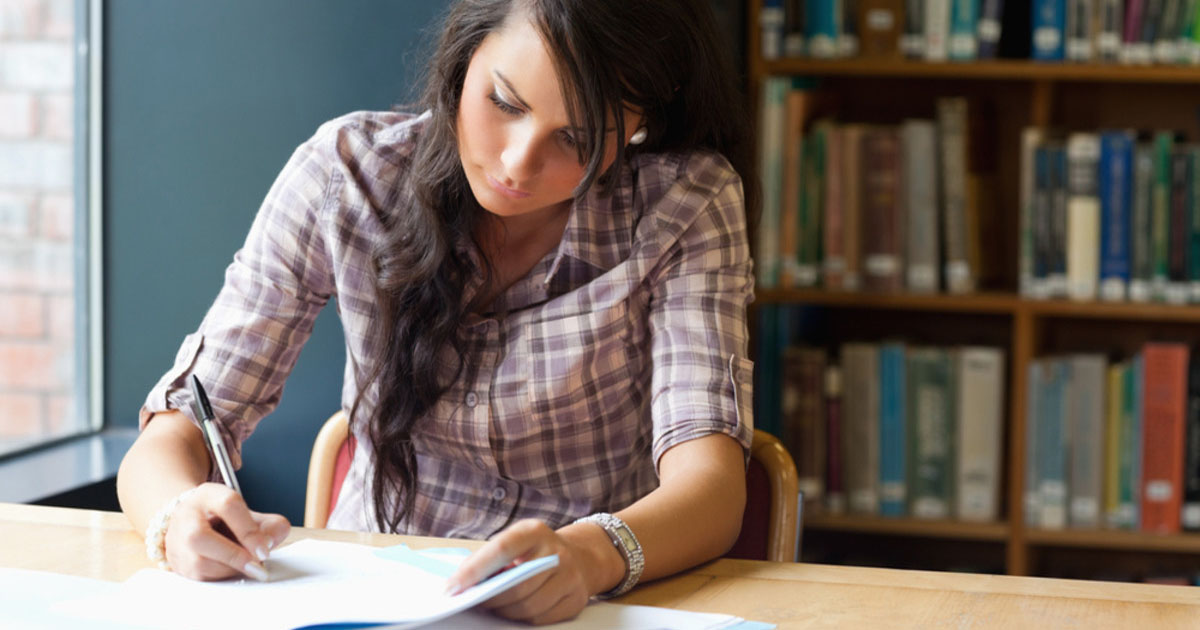
\includegraphics[width=1\textwidth]{Titelbild.png}
		%\cite{thirah_vorhangeschloss-schlussel-computer-icons_nodate}
		%\raggedleft
		\end{figure}
		
	
		\vfill
		
		\begin{normalsize}
			{
			\renewcommand\arraystretch{2}
			\begin{tabular}{>{\bf}p{4cm} l}
			Autoren   		           & Kim Schenk, Robin Aebi und	Gabriel Nussbaumer\\
			Dozent                 &    Tony Keller\\
			Modul		               &    Produktentwicklung und Innovation in der Elektrotechnik\\
			Hochschule                 &    Hochschule für Technik - FHNW\\
			Studiengang                &    Elektro- und Informationstechnik\\
%			Version                    &    1.0 %Normally not used!
			\end{tabular}
			}
		\end{normalsize}
	\end{center}
\clearpage
			
%%---ABSTRACT----------------------------------------------------------------------------
%\selectlanguage{english}				%ngerman or english
%\thispagestyle{empty}
%\include{sections/abstract}


%%---TABLE OF CONTENTS-------------------------------------------------------------------
\pagenumbering{Roman}		
\selectlanguage{ngerman}				%ngerman or english
\tableofcontents
\clearpage

%%---TEXT--------------------------------------------------------------------------------
\pagenumbering{arabic}

\clearpage
\section{Einleitung}\label{sec:Einleitung}
In dieser Bericht wird ein Essay über das Thema xxx erarbeitet. Der Bericht wird benotet und zählt als Abschlussarbeit für das Fach Produktentwicklung und Innovation in der Elektrotechnik, somit werden neben dem Essay, welches Zeit limitiert erarbeitet wird, noch zwei Innovationsmethoden beschrieben.\\
\newpage








%\clearpage
\section{6-3-5 Methode}\label{sec:635Methode}
Die 6-3-5 Methode ist eine Kreativitätstechnik zur Ideenfindung, optimalerweise wird Sie in einem Team mit 6 Personen angewendet. Es können Vorideen entstehen, wie auch gezielte Ideeanareicherung entwickelt werden.
\subsection{Vorgehensweise}
- In einem ersten Schritt werden Blätter in Papierform, jedem Teilenehmer verteilt, auf denen eine Tabelle mit 3 Spalten und die zuvor definierte Frage enthalten ist. Aus praktischen gründen sollten sich die Teilnehmer am selben Tisch befinden.\\
- Im zweiten Schritt sollte jeder Teilnehmer 3 Ideen zur Grundfrage, also meist eine Lösung für das definierte Problem, in je eine Spalte notieren. Die zeit zum nachdenken ist begrenzt auf 3 Minuten.\\
- In einem weiteren Schritt werden die Tabellen weitergegeben und die jeweils zuoberst beschriebenen Ideen können weiterentwickelt werden. Dieser Schritt wird im gesamten 5 mal durchgeführt.
\subsection{Vor- und Nachteile}
\begin{tabular}{|l|l|}
	\hline 
	Vorteile & Nachteile \\ 
	\hline 
	Jeder Teilnehmer kann seine Ideen & Keine Zeit für Fragen  \\
	 Notieren, keine dominanten Personen&\\ 
	\hline 
	Somit ist ein Protokoll erfasst&Es können Redundanzen entstehen \\ 
	\hline 
	Es entstehen in kurzer Zeit sehr viele&Arbeitstakt nicht für jeden Teilnehmer gleich\\
	interdisziplinäre Ideen&  \\ 
	\hline 
	Unnötige Diskussionen entfallen&Braucht eine Vorbereitung \\ 
	\hline 
	Jeder Teilnehmer muss sich beteiligen&  \\ 
	\hline 
\end{tabular} 
\subsection{Beispiel}
\begin{figure}[H]
	\centering
	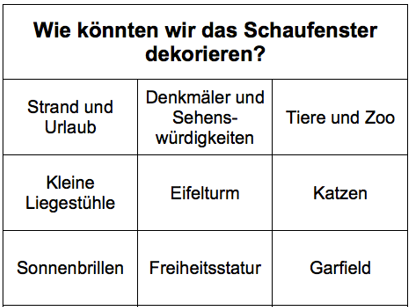
\includegraphics[width=0.5\textwidth]{M635.png}
	\caption{In dieser Abbildung kann erkannt werden, wie Ideen zur Frage: dekoration des Schafensters, entstanden sind}
	%\cite{thirah_vorhangeschloss-schlussel-computer-icons_nodate}
	%\raggedleft
\end{figure}

%\clearpage
\section{Brainstorming}\label{sec:Brainstorming}
\input{sections/Patent}
%\clearpage
\section{Claim-Chart}\label{sec:Claim-Chart}
%\clearpage
\section{Fazit}\label{sec:Fazit}
Mit dieser Arbeit konnte erkannt werden, dass verschiedene Patentierte Erfindungen von Palata, in dem zu analysierendem Gerät angewendet wurden. Das Patent Palata wurde verletzt und ein Patentanspruch kann abgehandelt werden. Wird in den Rechtsgrundlagen recherchiert kann zwischen unmittelbarer und mittelbarer Patentverletzung unterschieden werden. Bei unmittelbarer Patentverletzung ist alleine der Patentinhaber befugt, die patentierte Erfindung zu benutzen, was gesetzlich im Patentgesetz (PatG) verfasst ist. Bei der mittelbaren Patentverletzung erstreckt sich der Geltungsbereich der patentierten Erfindung noch weiter als bei den unmittelbaren Benutzungshandhabungen, es untersagt Dritten auch die Benutzung derjenige Mittel, die sich auf ein wesentliches Element der Erfindung beziehen.
\pagebreak


%\clearpage
%%---BIBLIOGRAPHY------------------------------------------------------------------------


{\sloppypar
%\printbibliography[heading=bibnumbered ]
\label{sec:lit}
\selectlanguage{ngerman}				%ngerman or english
\printbibliography
}

%\pagebreak

%\input{sections/8_0_Ehrlichkeitserklaerung}
%\pagebreak
%%---APPENDIX----------------------------------------------------------------------------
%\appendix
%%\begin{appendix} %Anhang


%Anhang A
%\includepdf[pages={1},nup=1x1,landscape=false,scale=0.90, pagecommand = \section*{\LARGE{Anhang:}}
%\addcontentsline{toc}{section}{Anhang}
%\section{Auftrag des Arbeitgebers}
%\label{app:Lastenheft}, offset =0mm -22mm ]{appendix/Lastenheft.pdf}\newpage
%Bei mehrseitigen Dokumenten die folgenden Seiten ohne Überschrift:
%\includepdf[pages={2},nup=1x1,landscape=false,scale=0.90,offset=6 -30,pagecommand={\thispagestyle{myheadings}}]{appendix/Lastenheft.pdf} 
%\newpage


%Anhang B: Bestimmung der Ersatzelemente der ASM
%\input{sections/ASM_Laborjournal}


%Anhang C: Messungen für ADC-Verifikation
\clearpage
\section{Messungen Zeitverzögerung Modulator}\label{app:Messungen_Delay Modulator}



\begin{figure}[H]
	\centering
	\includegraphics[width=0.85\linewidth]{appendix/Delay_modulator.png}
	\caption{Messung der Zeitverzögerung zwischen Modulatoreingang und modulierter Spannung an der ASM}
	\label{fig:app_delay}
\end{figure}


%Beispiel für A3 Seite einfügen:

%Anhang B
%A3
%\eject\pdfpagewidth=420mm \pdfpageheight=297mm
%A3


%Anhang B: Schema Layout
%\includepdf[pages={1},nup=1x1,landscape=false,scale=1.7,offset=300 -50,pagecommand={\section{Schema BMS-Slave}\label{app: Schema_Layout}\thispagestyle{myheadings}}]{appendix/Schema_Layout_.pdf} \newpage

%A4
%\eject\pdfpagewidth=210mm \pdfpageheight=297mm
%A4


%Beispiel Anhang C: (PDF)



%Anhang C: Dimensionierung passives Balancing
%\includepdf[pages={1},nup=1x1,landscape=false,scale=0.90,offset=10 -40,pagecommand={\section{Dimensionierung passives Balancing}\label{app: Dimensionierung_Balancing}\thispagestyle{myheadings}}]{appendix/Dimensionierung_Balancing.pdf} 
%\newpage


%\end{appendix}


%%---NOTES for DEBUG---------------------------------------------------------------------
%\ifdraft{%Do this only if mode=draft
%\usepackage{todonotes})
%\newpage
%\listoftodos[\section{Todo-Notes}]
%\clearpage
%}
%

\end{document}
